\documentclass{article}
\usepackage{amsmath, tikz, multicol, sfmath}
\tikzset{>=stealth}
\usetikzlibrary{calc}
\renewcommand{\familydefault}{\sfdefault}
\usepackage[margin = 0.5in]{geometry}
\pagestyle{empty}
\raggedright
\newcounter{Answers}
\begin{document}

\subsubsection*{Matrix Multiplication PSet \hfill Honors Algebra 2}

Given $\hat{\imath} = \begin{bmatrix} 1 \\ 0 \end{bmatrix}$ and $\hat{\jmath} = \begin{bmatrix} 0 \\ 1 \end{bmatrix}$, find \textbf{and graph} where $\hat{\imath}$ and $\hat{\jmath}$ end up after multiplying them by each matrix.

\begin{flalign*}
1.  \quad   &   A = \begin{bmatrix} -1 & 0 \\ 0 & -1 \end{bmatrix}   &
2.  \quad   &   B = \begin{bmatrix} -3 & 0 \\ 0 & -3 \end{bmatrix}   &
3.  \quad   &   C = \begin{bmatrix} 1 & -3 \\ 1 & 2 \end{bmatrix}   &
4.  \quad   &   D = \begin{bmatrix} 0 & 1 \\ 1 & 0 \end{bmatrix}    &&\\
\end{flalign*}

Describe, in words, the affect(s) that each of the following had on both $\hat{\imath}$ and $\hat{\jmath}$.   \newline\\

5. \quad Multiplying by $A$ in problem \#1 \qquad
6. \quad Multiplying by $B$ in problem \#2 \qquad
7. \quad Multiplying by $D$ in problem \#4 \\[0.3in]

Find each product (if possible) \textbf{and graph the result for 8 -- 12}.
\begin{flalign*}
8.  \quad   &   \begin{bmatrix} 2 & -2 \\ 1 & 0 \end{bmatrix}\begin{bmatrix} 1 \\ 1 \end{bmatrix}   &
9.  \quad   &   \begin{bmatrix} 3 & -1 \\ 1 & 2 \end{bmatrix}\begin{bmatrix} -4 \\ 0 \end{bmatrix}  &
10. \quad   &   \begin{bmatrix} -1 & 1 \\ 1 & -1 \end{bmatrix}\begin{bmatrix} -2 \\ 3 \end{bmatrix}   &
11. \quad   &   \begin{bmatrix} 0 & 3 \\ 1 & -2 \end{bmatrix}\begin{bmatrix} 4 & -1 \\ 2 & 0 \end{bmatrix}  &&\\[15pt]
12. \quad   &   \begin{bmatrix} 3 & 3 \\ -1 & 4  \end{bmatrix}\begin{bmatrix} -2 & 1 \\ -3 & -1  \end{bmatrix}   &
13. \quad   &   \begin{bmatrix} -4 & 5 & -5 \\ 5 & -2 & 0  \end{bmatrix}\begin{bmatrix} 3 & -3 \\ 1 & 4  \end{bmatrix} &
14. \quad   &   \begin{bmatrix} -4 & 5 \\ 5 & -2 \\ -5 & 0  \end{bmatrix}\begin{bmatrix} 3 & -3 \\ 1 & 4  \end{bmatrix} &
15. \quad   &   \begin{bmatrix} -5 & 5 & -4 \\ 2 & -3 & -4 \\ 5 & 5 & -2  \end{bmatrix}\begin{bmatrix} -3 \\ -1 \\ 1  \end{bmatrix}   &&\\
\end{flalign*}

\newpage

\textsc{Matrix Multiplication PSet Key}

\begin{multicols}{2}
\begin{enumerate}
    \item $\hat{\imath'} \to \begin{bmatrix} -1 \\ 0\end{bmatrix} \quad \hat{\jmath'} \to \begin{bmatrix} 0 \\ -1 \end{bmatrix}$  \newline\\   
    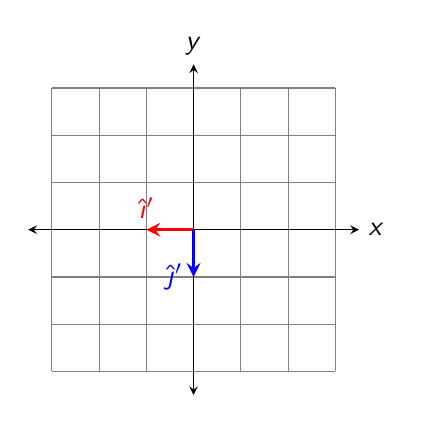
\begin{tikzpicture}[scale=0.6]
    \draw[gray] (-3,-3) grid (3,3);
    \draw[<->] (-3.5,0) -- (3.5,0) node [right] {$x$};
    \draw[<->] (0,-3.5) -- (0,3.5) node [above] {$y$};
    \draw[very thick, red, ->] (0,0) -- (-1,0) node [above] {$\hat{\imath}'$};
    \draw[very thick, blue, ->] (0,0) -- (0,-1) node [left] {$\hat{\jmath}'$};
    \end{tikzpicture}
    
    \item $\hat{\imath'} \to \begin{bmatrix} -3 \\ 0\end{bmatrix} \quad \hat{\jmath'} \to \begin{bmatrix} 0 \\ -3 \end{bmatrix}$  \newline\\   
    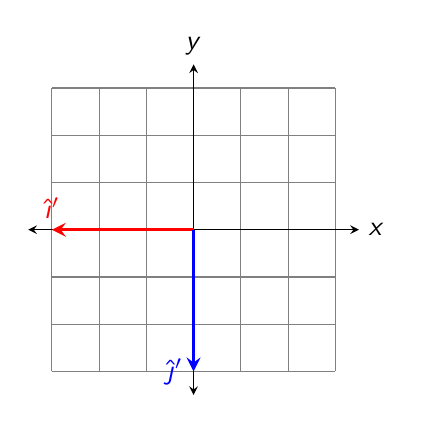
\begin{tikzpicture}[scale=0.6]
    \draw[gray] (-3,-3) grid (3,3);
    \draw[<->] (-3.5,0) -- (3.5,0) node [right] {$x$};
    \draw[<->] (0,-3.5) -- (0,3.5) node [above] {$y$};
    \draw[very thick, red, ->] (0,0) -- (-3,0) node [above] {$\hat{\imath}'$};
    \draw[very thick, blue, ->] (0,0) -- (0,-3) node [left] {$\hat{\jmath}'$};
    \end{tikzpicture}
\setcounter{Answers}{\value{enumi}}
\end{enumerate}
\end{multicols}

\begin{multicols}{2}
\begin{enumerate}
\setcounter{enumi}{\value{Answers}}
    \item $\hat{\imath'} \to \begin{bmatrix} 1 \\ 1\end{bmatrix} \quad \hat{\jmath'} \to \begin{bmatrix} -3 \\ 2 \end{bmatrix}$  \newline\\   
    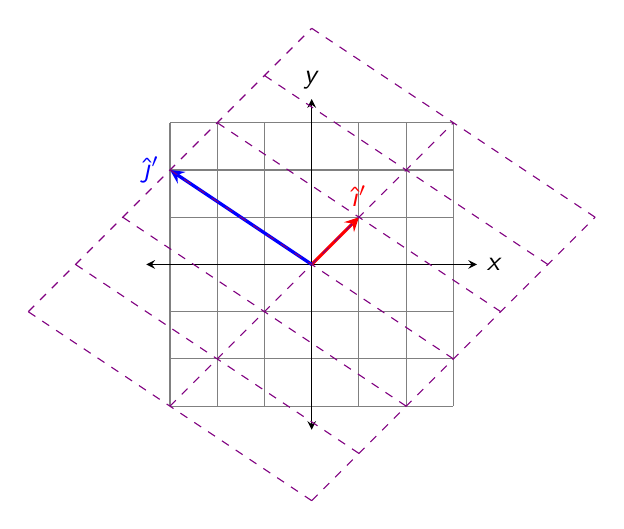
\begin{tikzpicture}[scale=0.6]
    \draw[gray] (-3,-3) grid (3,3);
    \draw[<->] (-3.5,0) -- (3.5,0) node [right] {$x$};
    \draw[<->] (0,-3.5) -- (0,3.5) node [above] {$y$};
    \draw[very thick, red, ->] (0,0) -- (1,1) node [above] {$\hat{\imath}'$};
    \draw[very thick, blue, ->] (0,0) -- (-3,2) node [left] {$\hat{\jmath}'$};
    \pgftransformcm{1}{1}{-3}{2}{\pgfpoint{0cm}{0cm}}
    \draw[dashed, violet] (-3,-1) grid (3,1);
    \end{tikzpicture}
    
    \item $\hat{\imath'} \to \begin{bmatrix} 0 \\ 1\end{bmatrix} \quad \hat{\jmath'} \to \begin{bmatrix} 1 \\ 0 \end{bmatrix}$  \newline\\   
    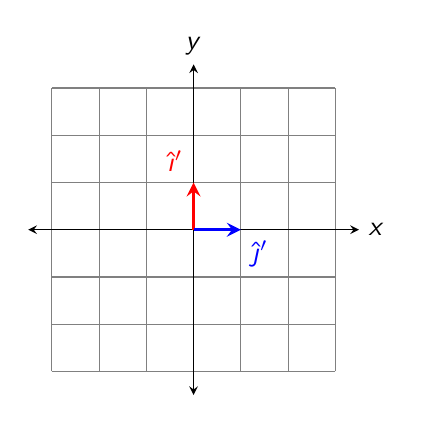
\begin{tikzpicture}[scale=0.6]
    \draw[gray] (-3,-3) grid (3,3);
    \draw[<->] (-3.5,0) -- (3.5,0) node [right] {$x$};
    \draw[<->] (0,-3.5) -- (0,3.5) node [above] {$y$};
    \draw[very thick, red, ->] (0,0) -- (0,1) node [above left] {$\hat{\imath}'$};
    \draw[very thick, blue, ->] (0,0) -- (1,0) node [below right] {$\hat{\jmath}'$};
    \end{tikzpicture}
\setcounter{Answers}{\value{enumi}}
\end{enumerate}
\end{multicols}

\begin{enumerate}
\setcounter{enumi}{\value{Answers}}
    \item \emph{Hint:} Graph $\hat{\imath}$ and $\hat{\jmath}$ on the same grid as your answer.
    
    \item \emph{Hint:} Graph $\hat{\imath}$ and $\hat{\jmath}$ on the same grid as your answer.
    
    \item \emph{Hint:} Graph $\hat{\imath}$ and $\hat{\jmath}$ on the same grid as your answer.
\setcounter{Answers}{\value{enumi}}
\end{enumerate}
    
\begin{multicols}{2}
\begin{enumerate}
\setcounter{enumi}{\value{Answers}}
    \item $\begin{bmatrix} 0 \\ 1 \end{bmatrix}$    \newline\\
    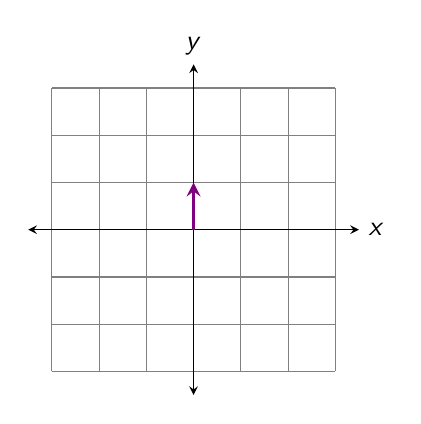
\begin{tikzpicture}[scale=0.6]
    \draw[gray] (-3,-3) grid (3,3);
    \draw[<->] (-3.5,0) -- (3.5,0) node [right] {$x$};
    \draw[<->] (0,-3.5) -- (0,3.5) node [above] {$y$};
    \draw[very thick, violet, ->] (0,0) -- (0,1);
    \end{tikzpicture}
    
    \item $\begin{bmatrix} -12 \\ -4 \end{bmatrix}$ \newline\\
    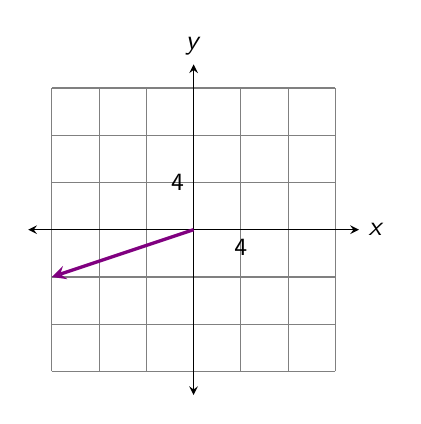
\begin{tikzpicture}[scale=0.6]
    \draw[gray] (-3,-3) grid (3,3);
    \draw[<->] (-3.5,0) -- (3.5,0) node [right] {$x$};
    \node at (1,0) [below] {\small 4};
    \node at (0,1) [left] {\small 4};
    \draw[<->] (0,-3.5) -- (0,3.5) node [above] {$y$};
    \draw[very thick, violet, ->] (0,0) -- (-3,-1);
    \end{tikzpicture}
\setcounter{Answers}{\value{enumi}}
\end{enumerate}
\end{multicols}

\newpage

\begin{multicols}{2}
\begin{enumerate}
\setcounter{enumi}{\value{Answers}}
    \item $\begin{bmatrix} 5 \\ -5 \end{bmatrix}$ \newline\\
    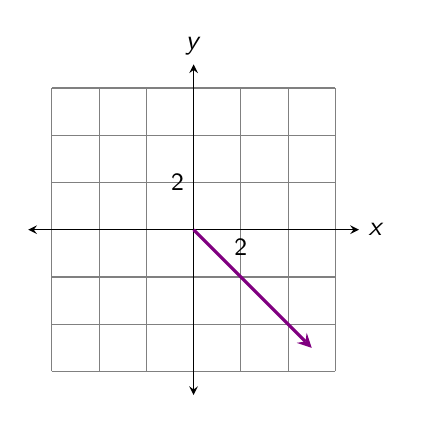
\begin{tikzpicture}[scale=0.6]
    \draw[gray] (-3,-3) grid (3,3);
    \draw[<->] (-3.5,0) -- (3.5,0) node [right] {$x$};
    \node at (1,0) [below] {\small 2};
    \node at (0,1) [left] {\small 2};
    \draw[<->] (0,-3.5) -- (0,3.5) node [above] {$y$};
    \draw[very thick, violet, ->] (0,0) -- (2.5,-2.5);
    \end{tikzpicture}
    
    \item $\begin{bmatrix} 6 & 0 \\ 0 & -1 \end{bmatrix}$   \newline\\
    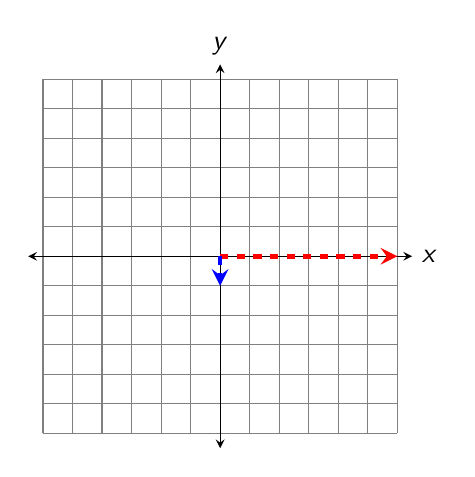
\begin{tikzpicture}[scale=0.375]
    \draw[gray] (-6,-6) grid (6,6);
    \draw[<->] (-6.5,0) -- (6.5,0) node [right] {$x$};
    \draw[<->] (0,-6.5) -- (0,6.5) node [above] {$y$};
    \draw[ultra thick, red, dashed, ->] (0,0) -- (6,0);
    \draw[ultra thick, blue, dashed, ->] (0,0) -- (0,-1);
    \end{tikzpicture}
\setcounter{Answers}{\value{enumi}}
\end{enumerate}
\end{multicols}

\begin{enumerate}   \setlength\itemsep{20pt}
\setcounter{enumi}{\value{Answers}}
    \item $\begin{bmatrix} -15 & 0 \\ -10 & -5 \end{bmatrix}$ \newline\\
    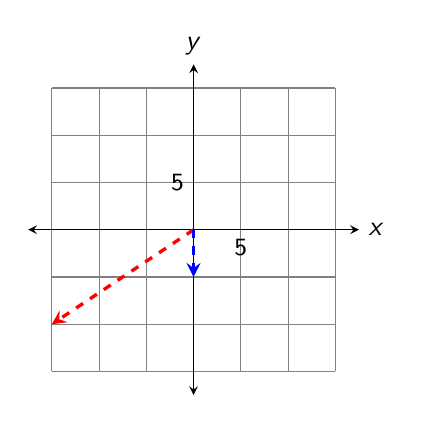
\begin{tikzpicture}[scale=0.6]
    \draw[gray] (-3,-3) grid (3,3);
    \draw[<->] (-3.5,0) -- (3.5,0) node [right] {$x$};
    \node at (1,0) [below] {\small 5};
    \node at (0,1) [left] {\small 5};
    \draw[<->] (0,-3.5) -- (0,3.5) node [above] {$y$};
    \draw[very thick, red, dashed, ->] (0,0) -- (-3,-2);
    \draw[very thick, blue, dashed, ->] (0,0) -- (0,-1);
    \end{tikzpicture}
    
    \item Not possible
    
    \item $\begin{bmatrix} -7 & 32 \\ 13 & -23 \\ -15 & 15 \end{bmatrix}$
    
    \item $\begin{bmatrix} 6 \\ -7 \\ -22 \end{bmatrix}$
\end{enumerate}
\end{document}
